\documentclass[11pt]{article}

\usepackage{mathtools}
\usepackage{amssymb}
\usepackage[latin1]{inputenc}
\usepackage[margin=0.5in]{geometry}
\usepackage{graphicx}

\everymath{\displaystyle}
\setlength\parindent{0pt}

\begin{document}
\title{Stanford CS 229, Public Course, Problem Set 2}
\date{\today}
\author{Dylan Price}
\maketitle 

% custom commands
\newcommand{\half}[0]{\frac{1}{2}}
\newcommand{\pder}[2]{\frac{\partial#1}{\partial#2}}
\newcommand{\thetaT}[0]{\theta^{T}}
\newcommand{\ith}[1]{#1^{(i)}}
\newcommand{\xith}[0]{\ith{x}}
\newcommand{\yith}[0]{\ith{y}}
\newcommand{\sumitom}[0]{\sum_{i=1}^{m}}
\newcommand{\xnew}[0]{x_{new}}

\section{}

\subsection*{a)}

Find a closed-form expreesion for the value of $\theta$ which minimizes the ridge regression cost function:

$J(\theta) = \half \sumitom (\thetaT \xith - \yith)^{2} + \frac{\lambda}{2}\|\theta\|^{2}$ \\ \\

First, put $J(\theta)$ into matrix notation
\begin{align*}
  J(\theta) &= \half \sumitom (\thetaT \xith - \yith)^{2} + \frac{\lambda}{2}\|\theta\|^{2} \\
            &= \half \sumitom (\thetaT \xith - \yith)(\thetaT \xith - \yith) + \frac{\lambda}{2}\|\theta\|^{2} \\
            &= \half (X \theta - \vec{y})(X \theta - \vec{y}) + \frac{\lambda}{2} \thetaT \theta \\
            & \text{(where $X$ is the design matrix and $\vec{y}$ is the vector of target values)} \\
            &= \half ((X \theta)^{T} X \theta - (X \theta)^{T} \vec{y} - \vec{y}^{T} X \theta + \vec{y}^{T} \vec{y})) + \frac{\lambda}{2} \thetaT \theta \\
            &= (\half \thetaT X^{T} X \theta - \half \thetaT X^{T} \vec{y} - \half \vec{y}^{T} X \theta + \half \vec{y}^{T} \vec{y}) + \frac{\lambda}{2} \thetaT \theta \\
\end{align*}


Now find the gradient
\begin{align*}
  \nabla_{\theta} J(\theta) &= X^{T} X \theta - \half X^{T} \vec{y} - \half X^{T} \vec{y} + \lambda \theta \\
  &= X^{T} X \theta - X^{T} \vec{y} + \lambda \theta \\
\end{align*}

Set the gradient equal to $0$ and solve for $\theta$
\begin{align*}
  X^{T} X \theta - X^{T} \vec{y} + \lambda \theta &= 0 \\
  X^{T} X \theta + \lambda \theta &= X^{T} \vec{y} \\
  (X^{T} X + \lambda I) \theta &= X^{T} \vec{y} \\
  \theta &= (X^{T} X + \lambda I)^{-1} X^{T} \vec{y} \\
\end{align*}

\subsection*{b)}

Suppose that we want to use kernels to implicitly represent our feature vectors in a high-dimensional (possibly infinite dimensional) space. 

Making a prediction on a new input $\xnew$ would now be done by computing $\thetaT \phi(\xnew)$.

Show how we can use the "kernel trick" to obtain a closed form for the prediction on the new input without ever explicitly computing $\phi(\xnew)$.

\begin{align*}
  h_{\theta}(\xnew) &= \thetaT \xnew \\
             &= ((X^{T} X + \lambda I)^{-1} X^{T} \vec{y})^{T} \xnew \\
             &= ((X X^{T} + \lambda I)^{-1} \vec{y})^{T} X \xnew \\
             &= \vec{y}^{T} (X X^{T} + \lambda I)^{-T} X \xnew \\
\end{align*}

Now we replace $\xith$ with $\phi(\xith)$ for $i = 1...m$,\\
define kernel function $K(x, z) = \phi(x) \phi(z)$ \\
and kernel matrix $K \in \mathbb{R}^{m x m}$ such that $K_{ij} = K(\xith, x^{(j)})$

\begin{align*}
  h_{\theta}(\xnew) &= \vec{y}^{T} (K + \lambda I)^{-T} \sumitom K(\xith, \xnew) \\
\end{align*}

\section*{2}

\begin{align*}
  \underset{w,b,\xi}{\text{min}} &\quad \half \|w\|^{2} + \frac{C}{2} \sumitom \xi_{i}^{2} \\
  \text{subject to} &\quad \yith (w^{T} \xith + b) \geq 1 - \xi_i, i = 1,...,m \\
\end{align*}

\subsection*{a)}

Notice that we have dropped the $\xi_{i} \geq 0$ constraint in the $\ell_2$ problem. Show that these non-negativity constraints can be removed. That is, show that the optimal value of the objective will be the same whether or not these constraints are present. \\

Let $\xi_i$ be a negative error in $\xi_0,...,\xi_m$. Since $\xi_i^{2}$ is positive, $\xi_i$ will contribute the same amount to the objective as $-\xi_i$. Therefore the minimization of the objective does not depend on the sign of $\xi_i$ and the $\xi_i \geq 0$ constraint is irrelevant.

\subsection*{b)}

What is the Lagrangian of the $\ell_2$ soft margin SVM optimization problem?

Let
\begin{align*}
  f(w)   &= \half \|w\|^{2} + \frac{C}{2} \sumitom \xi_i^2 \\
  g_i(w) &= -\yith (w^T \xith + b) + 1 - \xi_i \\
\end{align*}

Our optimization problem is
\begin{align*}
  \text{min}        &\quad f(w) \\
  \text{subject to} &\quad g_i(w) \geq 0, i = 1,...,m \\
\end{align*}

The Lagrangian is
\begin{align*}
  \mathcal{L}(w,b,\alpha,\xi) &= f(w) + \sumitom \alpha_i g_i(w) \\
  &= \half \|w\|^2 + \frac{C}{2} \sumitom \xi_i^2 + \sumitom \alpha_i (-\yith (w^T \xith + b) + 1 - \xi_i) \\
  &= \half w^T w + \frac{C}{2} \xi^T \xi + \sumitom \alpha_i (-\yith w^T \xith - \yith b + 1 - \xi_i) \\
  &= \half w^T w + \frac{C}{2} \xi^T \xi - \sumitom \alpha_i \yith w^T \xith - \sumitom \alpha_i \yith b + \sumitom \alpha_i - \sumitom \alpha_i \xi_i \\
\end{align*}

\subsection*{c)}

Minimize the Lagrangian with respect to $w$, $b$, and $\xi$ by taking the following gradients: $\nabla_w \mathcal{L}$, $\pder{\mathcal{L}}{b}$, and $\nabla_{\xi} \mathcal{L}$, and then setting them equal to $0$. Here $\xi = |\xi_1,\xi_2,...,\xi_m|^{T}$. \\

First find $\nabla_w \mathcal{L}$
\begin{align*}
  \nabla_w \mathcal{L} &= w + \sumitom -\alpha_i \yith \xith \\
                       &= w - \sumitom \alpha_i \yith \xith \\
\end{align*}

Set equal to 0
\begin{align*}
                     0 &= w - \sumitom \alpha_i \yith \xith \\
                     w &= \sumitom \alpha_i \yith \xith \\
\end{align*}

Next find $\pder{\mathcal{L}}{b}$
\begin{align*}
  \pder{\mathcal{L}}{b} &= \sumitom -\alpha_i \yith \\
\end{align*}

Set equal to 0
\begin{align*}
  0 &= \sumitom -\alpha_i \yith \\
  0 &= \sumitom \alpha_i \yith \\
\end{align*}

Find $\nabla_{\xi} \mathcal{L}$
\begin{align*}
  \nabla_{\xi} \mathcal{L} &= C \xi - \alpha \\
\end{align*}

Set equal to 0
\begin{align*}
  0   &= C \xi - \alpha \\
  \xi &= \frac{1}{C} \alpha \\
\end{align*}

Plug these results back into the Lagrangian
\begin{align*}
  \mathcal{L}(w,b,\alpha,\xi) &= \half w^T w + \frac{C}{2} \xi^T \xi - \sumitom \alpha_i \yith w^T \xith - \sumitom \alpha_i \yith b + \sumitom \alpha_i - \sumitom \alpha_i \xi_i \\
  \underset{w,b,\xi}{min} \quad \mathcal{L} &= \half (\sumitom \alpha_i \yith \xith)^T (\sumitom \alpha_i \yith \xith) + \frac{C}{2} (\frac{1}{C} \alpha)^T (\frac{1}{C} \alpha) \\
                                            &\quad - \sumitom \alpha_i \yith (\sum_{j=1}^{m} \alpha_j y^{(j)} x^{(j)})^T \xith - \sumitom \alpha_i \yith b + \sumitom \alpha_i - \sumitom \alpha_i (\frac{1}{C} \alpha_i) \\
                                            &= \half \sumitom \sum_{j=1}^{m} \alpha_i \alpha_j \yith y^{(j)} (\xith)^T x^{(j)} + \frac{1}{2C} \alpha^T \alpha \\
                                            &\quad - \sumitom \sum_{j=1}^{m} \alpha_i \alpha_j \yith y^{(j)} (\xith)^T x^{(j)} - \sumitom \alpha_i \yith b + \sumitom \alpha_i - \sumitom \frac{1}{C} \alpha_i^2 \\ 
                                            &= \half \sumitom \sum_{j=1}^{m} \alpha_i \alpha_j \yith y^{(j)} (\xith)^T x^{(j)} + \frac{1}{2C} \sumitom \alpha_i^2 \\
                                            &\quad - \sumitom \sum_{j=1}^{m} \alpha_i \alpha_j \yith y^{(j)} (\xith)^T x^{(j)} - \sumitom \alpha_i \yith b + \sumitom \alpha_i - \frac{1}{C} \sumitom \alpha_i^2 \\ 
                                            &= -\half \sumitom \sum_{j=1}^{m} \alpha_i \alpha_j \yith y^{(j)} (\xith)^T x^{(j)} - b \sumitom \alpha_i \yith + \sumitom \alpha_i - \frac{1}{2C} \sumitom \alpha_i^2 \\
                                            &\text{From above we know that $0 = \sumitom \alpha_i \yith$ when the Lagrangian is minimized, so we end with} \\
  \underset{w,b,\xi}{min} \quad \mathcal{L} &= -\half \sumitom \sum_{j=1}^{m} \alpha_i \alpha_j \yith y^{(j)} (\xith)^T x^{(j)} + \sumitom \alpha_i - \frac{1}{2C} \sumitom \alpha_i^2 \\
\end{align*}
\subsection*{d)}

What is the dual of the $\ell_2$ soft margin SVM optimization problem?

\begin{align*}
  \underset{\alpha}{max} &\quad \theta_D \\
  \text{subject to}      &\quad \sumitom \alpha_i \yith = 0 \\
                         &\quad \alpha_i \geq 0, i=1,...,m \\
                         \\
  \text{where}           &\quad \theta_D = \underset{w,b,\xi}{min} \quad \mathcal{L} \text{, which we found above} \\
\end{align*}

\section*{3}

\subsection*{a)}

$f(x) = \sumitom \alpha_i \yith K(\xith,x) + b  \quad ; \quad  K(x,z) = exp(\frac{-||x-z||^2}{\tau^2})$

Find values for the set of parameters $\{\alpha_1,...,\alpha_m,b\}$ and Gaussian kernel width $\tau$ such that $\xith$ is correctly classified for all $i = 1,...,m$. \\\\

Let $\alpha_i = 1, b = 0$ for $i = 1,...,m$. Then \\

$f(x) = \sumitom \yith e^{\frac{-||\xith - x||^2}{\tau^2}}$ \\

Find $\tau$ such that $|f(\xith) - \yith| < 1$ for all $i$.

\begin{align*}
    |f(\xith) - \yith| &= |\sum_{j=1}^{m} y^{(j)} e^{\frac{-||x^{(j)} - \xith||^2}{\tau^2}|} - y^{(i)}| \\
                       &= |\yith e^{\frac{-||\xith - \xith||^2}{\tau^2}} + \sum_{j \ne i} y^{(j)} e^{\frac{-||x^{(j)} - \xith||^2}{\tau^2}} - \yith| \\
                       &= |\sum_{j \ne i} y^{(j)} e^{\frac{-||x^{(j)} - \xith||^2}{\tau^2}}| \\
                       &\le \sum_{j \ne i} | \yith e^{\frac{-||x^{(j)} - \xith||^2}{\tau^2}}| &\text{By the triangle inequality} \\
                       &= \sum_{j \ne i} | e^{\frac{-||x^{(j)} - \xith||^2}{\tau^2}}| &\text{$\yith \in \{-1,1\},$ so $|\yith| = 1$} \\
                       &\le \sum_{j \ne i} | e^{\frac{-\epsilon^2}{\tau^2}}| &\text{$||x^{(j)} - \xith|| \ge \epsilon$ when $i \ne j$} \\
                       &= (m-1) e^{\frac{-\epsilon^2}{\tau^2}} \\
\end{align*}
\begin{align*}
                  \text{Now we set this} &< 1 \\
    (m-1) e^{\frac{-\epsilon^2}{\tau^2}} &< 1 \\
          e^{\frac{-\epsilon^2}{\tau^2}} &< \frac{1}{m-1} \\
     \log e^{\frac{-\epsilon^2}{\tau^2}} &< \log \frac{1}{m-1} \\
            \frac{-\epsilon^2}{\tau^2}  &< \log  \frac{1}{m-1} \\
            \frac{\epsilon^2}{\tau^2}   &> - \log  \frac{1}{m-1} \\
            \frac{\epsilon^2}{\tau^2}   &> \log(m-1) \\
           \frac{\epsilon^2}{\log(m-1)} &> \tau^2 \\
    \sqrt{\frac{\epsilon^2}{\log(m-1)}} &> \tau \\
                                   \tau &< \frac{\epsilon}{\sqrt{\log(m-1)}} \\
\end{align*}

\subsection*{b)}
Yes, if we run an SVM without slack variables using the parameter $\tau$ from part (a), the resulting classifier will obtain zero training error. Zero training error corresponds to perfectly separating the training data, which is what an SVM without slack variables will do. Since our value of $\tau$ guarantees the training data to be separable, our classifier will obtain zero training error.

\subsection*{c)}
No, if we run the SMO algorithm with slack variables the resulting classifier will not necessarily obtain zero training error. The parameter C controls how much we penalize the slack terms ($\xi_i$) and if we don't penalize slack enough then a smaller value for the objective function may be achieved by introducing a lot of slack and not necessarily by achieving zero training error.

\section*{4}
Below is the graph I produced running weka against all the training sets. The x axis is number of training samples, while the y axis is percentage of incorrectly classified instances. The blue line is the NaiveBayesMultinomial classifier while the green line is the SMO classifier.

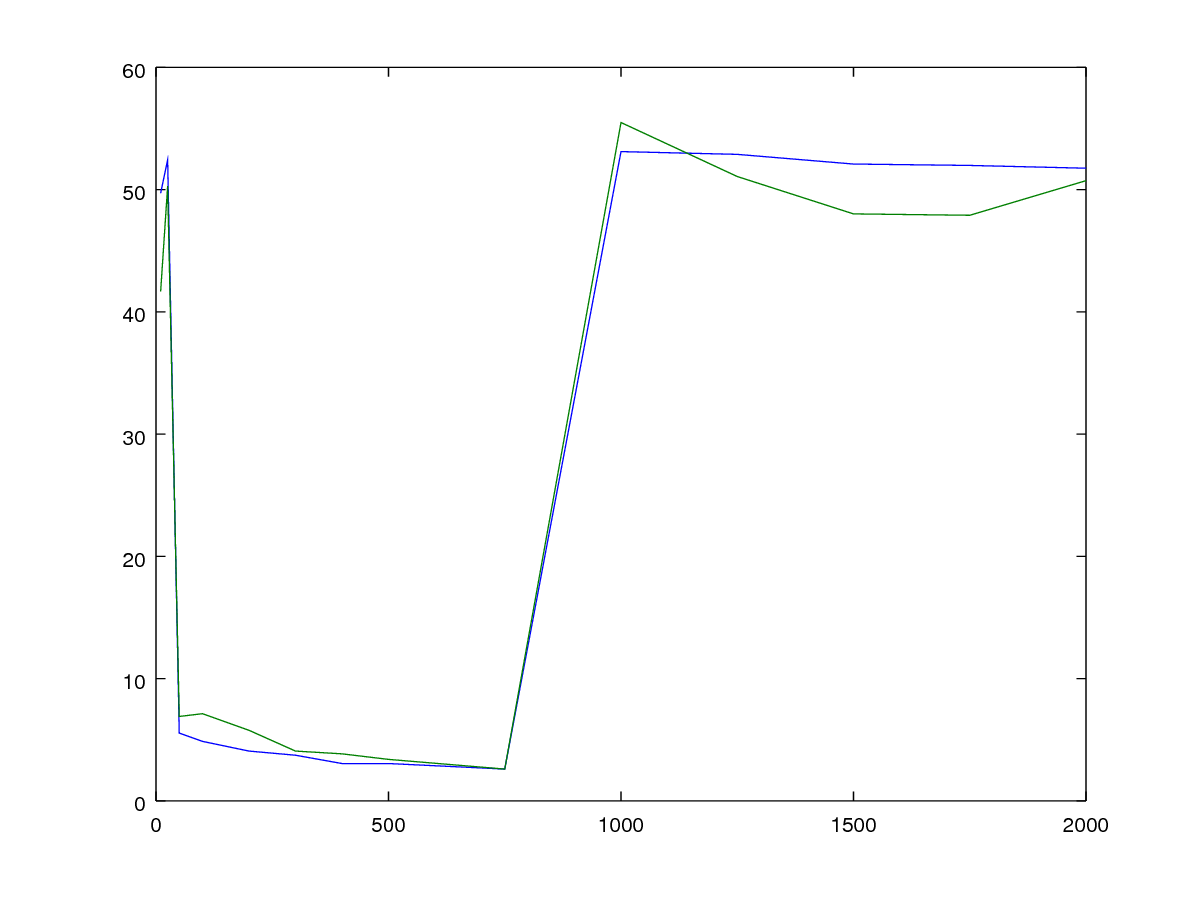
\includegraphics[width=\textwidth]{q4/num_examples_vs_error.png}

The result I expected is that both algorithms would improve as the number of training examples increased, with perhaps one outperforming the other. As you can see, something is likely wrong with the training data or with how I am running weka against it. 

\section*{5}

\end{document}
